\documentclass[11pt,letterpaper]{report}
\usepackage{amssymb,amsfonts,color,graphicx,amsmath,enumerate}
\usepackage{amsthm}

\newcommand{\naturals}{\mathbb{N}}
\newcommand{\integers}{\mathbb{Z}}
\newcommand{\complex}{\mathbb{C}}
\newcommand{\reals}{\mathbb{R}}
\newcommand{\mcal}[1]{\mathcal{#1}}
\newcommand{\rationals}{\mathbb{Q}}
\newcommand{\field}{\mathbb{F}}
\newcommand{\Var}{\text{Var}}
\newcommand{\ind}{\mathbbm{1}}
\newcommand{\Cov}{\text{Cov}}
\newcommand{\diam}{\text{diam}}
\newcommand{\subg}[1]{\left\|{#1}\right\|_{\psi_2}}
\newcommand{\Lp}[2]{\left\|{#1}\right\|_{L^{#2}}}
\newcommand{\Lip}[1]{\left\|{#1}\right\|_{\text{Lip}}}
\newcommand{\Unif}{\text{Unif}}
\newcommand{\tr}{\text{tr}}
\newcommand{\vc}{\text{vc}}

\newenvironment{solution}
{\begin{proof}[Solution]}
{\end{proof}}

\voffset=-3cm
\hoffset=-2.25cm
\textheight=24cm
\textwidth=17.25cm
\addtolength{\jot}{8pt}
\linespread{1.2}

\begin{document}
\noindent{\em Liam Hardiman\hfill{June 4, 2020} }
\begin{center}
{\bf \Large 270C - Homework 4}
\vspace{0.2cm}
\hrule
\end{center}

%7.2.6, 7.3.5, 7.4.2, 8.1.7, 8.1.12 (this exercise is about the canonical process, see Definition 7.5.1), 8.2.6, 8.3.5, 8.3.7, 8.3.15, 8.3.17, 8.3.24, 8.3.25, 8.4.6(ignore), 8.4.8.

\section*{7.2.6}
Let $X\sim \mcal{N}(0, \Sigma)$. Show that for any differentiable function $f:\reals^n\to \reals$ we have
\[
E[Xf(X)] = \Sigma\cdot E[\nabla f(X)]
\]
\begin{proof}
	Zooming in on each coordinate shows that the conclusion is equivalent to
	\[
	E[X_if(X)] = \sum_{j=1}^n\Sigma_{ij}E\big[\partial_{x_j}f(X)\big],\quad i=1, \ldots, n.
	\]
	Write $X = \Sigma^{1/2}Z$ for $Z\sim \mcal{N}(0, I_n)$. We then have that
	\[
	E[X_i f(X)] = \sum_{k=1}^n(\Sigma^{1/2})_{ik}E\big[Z_kf(\Sigma^{1/2}Z)\big].
	\]
	Now we evaluate the expectation under the sum by conditioning on $Z_j$, $j\neq k$ and applying univariate Gaussian integration by parts (conditioning turns the multivariable function $f(\Sigma^{1/2}Z)$ into a single variable function). By the chain rule we have
	\begin{align*}
		(\Sigma^{1/2})_{ik}E\big[Z_kf(\Sigma^{1/2}Z)\big] &= (\Sigma^{1/2})_{ik}E\bigg[E\big[Z_kf(\Sigma^{1/2}Z)\mid Z_i,\ i\neq k\big]\bigg]\\
		&= (\Sigma^{1/2})_{ik}E\big[(\Sigma^{1/2})_{ik}\partial_{x_k}f(\Sigma^{1/2}Z)\big].
	\end{align*}
\end{proof}










\section*{7.3.5}
Let $A$ be a symmetric $n\times n$ Gaussian random matrix whose entries above the diagonal are independent $\mcal{N}(0, 1)$ random variables, and the diagonal entries are independent $\mcal{N}(0, 2)$ random variables. Show that
\[
E\|A\| \leq 2\sqrt{n}.
\]
Then deduce the tail bound
\[
\Pr\big[\|A\|\geq 2\sqrt{n}+t\big]\leq 2\exp(-ct^2).
\]
\begin{proof}
	We adapt the proof of theorem 7.3.1 to work for symmetric matrices. We start by realizing the norm of $A$ as the supremum of a Gaussian process.
	\[
	\|A\| = \max_{u\in S^{n-1}}\langle Au, u\rangle = \max_{u\in S^{n-1}}X_u,
	\]
	where $X_u = \langle Au, u\rangle \sim \mcal{N}(0, 1)$. We aim to apply Sudakov-Fernique, so we compute the second moment of the increments of $X$.
	\begin{align*}
		E(X_u-X_v)^2 &= E\big[\langle Au, u\rangle - \langle Av, v\rangle\big]\\
		&= E\left(\sum_{i,j}A_{ij}(u_iu_j - v_iv_j)\right)^2.
	\end{align*}
	By independence and symmetry, this quantity is equal to
	\begin{align*}
		2\sum_{i=1}^n(u_i^2-v_i^2)^2 + \sum_{i,j,k,l}E[A_{ij}A_{kl}](u_iu_j-v_iv_j)(u_ku_l-v_kv_l) &= 2\sum_{i=1}^n(u_i^2-v_i^2)^2 + 2\sum_{i<j}(u_iu_j-v_iv_j)^2\\
		&= 2\|uu^T-vv^T\|_F^2\\
		&\leq 2\|u-v\|_2^2.
	\end{align*}
	Consider the process $Y_u = \sqrt{2}\langle g, u\rangle$, where $g\sim \mcal{N}(0, I_n)$ and $u\in S^{n-1}$. The increments of this process satisfy
	\[
	E(Y_u-Y_v)^2 = 2E[\langle g, u-v\rangle^2] = 2\|u-v\|_2^2.
	\]
	We have what we need to apply Sudakov-Fernique:
	\begin{align*}
		E\|A\| &= E\sup_{u\in S^{n-1}}X_u \leq E\sup_{u\in S^{n-1}}Y_u\\
		&= \sqrt{2}E\|g\|_2\\
		&\leq \sqrt{2}(E\|g\|_2^2)^{1/2}\\
		&= \sqrt{2n}
	\end{align*}
	As for the tail bound, we follow the proof of corollary 7.3.3 with some modifications. The proof of that corollary doesn't immediately work here since our matrix $A$, when viewed as a vector in $\reals^{n^2}$ isn't a standard normal random vector, so we can't apply theorem 5.2.2.. Instead, we apply the fancier theorem 5.2.15. The density function for our vector $A$, $\rho$, has the form
	\[
	\rho(x) = \exp\left(-\frac{1}{2}x^T\Sigma x + c\right) = \exp(-U(x)),
	\]
	where $c$ is a constant that depends only on $n$ and $\Sigma$ is an $n^2\times n^2$ covariance matrix. The Hessian of $U$ is $\frac{1}{2}\Sigma$, whose eigenvalues (I want to say) are bounded below by an absolute constant, $\kappa$. By theorem 5.2.15, if $f(A) = \|A\|$, then since $f(A)\leq \|A\|_2$ and $\Lip{f} \leq 1$, we have
	\[
	\subg{f(A)-Ef(A)}\leq C\frac{\Lip{f}}{\sqrt{\kappa}}\leq \frac{C}{\sqrt{\kappa}}.
	\]
	Since this upper bound is an absolute constant, the desired tail bound follows.
\end{proof}










\section*{7.4.2}
Show that if $(T, d)$ is not totally bounded, that is if $N(T, d, \epsilon)=\infty$ for some $\epsilon>0$, then
\[
E \sup_{t\in T}X_t = \infty,
\]
where $X_t$ is a mean zero Gaussian process and $d$ is the canonical metric determined by $X$.
\begin{proof}
	We basically copy the proof of Sudakov's minoration inequality up to the last step. Let $\epsilon>0$ be such that $N(T, d, \epsilon) = \infty$ and take a maximal $\epsilon$-separated subset of $T$, $\mcal{N}$. We restrict our process $X$ to $\mcal{N}$ and compare it to the process $(Y_t)_{t\in \mcal{N}}$,
	\[
	Y_t = \frac{\epsilon}{\sqrt{2}}g_t,\quad g_t\sim \mcal{N}(0, 1)\text{ iid.}
	\]
	We compare the increments of our processes:
	\[
	E(X_t - X_s)^2 = d(t, s)^2 \geq \epsilon^2,\qquad E(Y_t-Y_s)^2 = \frac{\epsilon^2}{2}E(g_t-g_2)^2= \epsilon^2.
	\]
	Since $E(X_t-X_s)^2 \geq E(Y_t-Y_s)^2$ for all $s,t\in \mcal{N}$, by Sudakov-Fernique we have
	\[
	E\sup_{t\in \mcal{N}}X_t \geq E\sup_{t\in \mcal{N}}Y_t = \frac{\epsilon}{2}\cdot E\max_{t\in \mcal{N}}g_t.
	\]
	Since $\mcal{N}$ is infinite, it suffices to show that the expected maximum of infinitely many iid standard normal random variables is infinite. This follows from the monotonicity of expectation and the fact that $E\sup_{i\leq N}g_i \geq c\sqrt{\log N}$. Specifically, let $\mcal{N}_n$ be any set of $n$ points in $N$. For any $n$ we have that
	\[
		E\sup_{t\in \mcal{N}}g_t \geq E\sup_{t\in \mcal{N}_n}g_t \geq c\sqrt{\log n}.
	\]
	Since $|\mcal{N}| = \infty$, taking the limit as $n\to \infty$ gives the desired result.
\end{proof}










\section*{8.1.7}
Let $(X_t)_{t\in T}$ be a random process on a metric space $(T, d)$ with sub-gaussian increments, i.e. for some $K\geq 0$
\[
\subg{X_t-X_s}\leq Kd(t,s)\quad\text{for all }s,t\in T.
\]
Show that for every $u\geq 0$, the event
\[
\sup_{s,t\in T}|X_t-X_s|\leq CK\left(\int_0^\infty\sqrt{\log N(T, d, \epsilon)}d\epsilon + u\cdot \diam(T)\right)
\]
holds with probability at least $1-2\exp(-u^2)$.
\begin{proof}
	Fix $t\in T$ and a positive integer $k$. Recall that
	\[
	\subg{X_{\pi_{k}(t)}-X_{\pi_{k-1}(t)}}\leq c\epsilon_{k-1}
	\]
	A union bound over $T$ then gives
	\begin{align*}
		\Pr\left[\sup_{t\in T} (X_{\pi_k(t)}-X_{\pi_{k-1}(t)})\geq C\epsilon_{k-1}(\sqrt{\log|T_k|}+z)\right] &\leq |T_k|\exp\left(-\frac{C^2\epsilon_{k-1}^2(\sqrt{\log |T_k|}+z)^2}{c^2\epsilon_{k-1}^2}\right)\\
		&\leq |T_k|\exp[-C'(\log|T_k|+z^2)]\\
		&= |T_k|^{1-C'}e^{-C'z^2}\\
		&\leq e^{-z^2},
	\end{align*}
	for $C'>1$. Union bounding over $k$ gives
	\[
	\Pr\left[\sup_{t\in T}(X_{\pi_k(t)}-X_{\pi_{k-1}(t)}) > C\epsilon_{k-1}(\sqrt{\log|T_k|} + z_k)\text{ for some }k\right] \leq \sum_{k=\kappa}^\infty e^{-z_k^2},
	\]
	where $\kappa$ is the largest integer such that $\epsilon_{\kappa} \geq \diam(T)$. Fix some $t_0\in T$. Since $\kappa$ is independent of $t_0$, summing over $k$ gives
	\[
	\Pr\left[\sup_{t\in T}|X_t-X_{t_0}| > C\left(\int_0^\infty \sqrt{\log N(T, d, \epsilon)}d\epsilon + \sum_{k=\kappa}^\infty\epsilon_{k-1}z_k\right) \right]\leq \sum_{k=\kappa}^\infty e^{-z_k^2}.
	\]
	Now we set $z_k = u+\sqrt{k-\kappa+1}$. This gives
	\[
	\sum_{k=\kappa}^\infty \epsilon_{k-1}z_k = \epsilon_\kappa u\sum_{k=\kappa}^\infty 2^{-k}\sqrt{k-\kappa+1}\geq u\cdot \diam(T).
	\]
	Bounding the sum of a geometric series by twice its first term gives
	\[
	\sum_{k=\kappa}^\infty e^{-z_k^2} = \sum_{k=\kappa}^\infty e^{-u^2(k-\kappa+1)} \leq 2e^{-u^2}.
	\]
	From this, we deduce
	\[
	\Pr\left[\sup_{t\in T}|X_t-X_{t_0}| > C\left(\int_0^\infty \sqrt{\log N(T, d, \epsilon)}d\epsilon + u\cdot \diam (T)\right) \right]\leq 2e^{-u^2},
	\]
	as desired.
\end{proof}










\section*{8.1.12}
Let $e_1, \ldots, e_n$ be the canonical basis vectors in $\reals^n$. Consider the set
\[
T = \left\{\frac{e_k}{\sqrt{1+\log k}},\ k=1, \ldots, n\right\}.
\]
\begin{enumerate}[(a)]
	\item Show that
	\[
	w(T)\leq C,
	\]
	where as usual, $C$ is an absolute constant and $w(T)$ is the Gaussian width
	\[
	w(T) = E\sup_{x\in T}\langle g, x\rangle\quad\text{where }g\sim \mcal{N}(0, I_n).
	\]
	\begin{proof}
		If $g\sim \mcal{N}(0, I_n)$ then $\langle g, e_k\rangle \sim \mcal{N}(0, 1)$. By exercise 2.5.10 (old homework problem), we have
		\[
		E \max_k \frac{\langle g, e_k\rangle}{\sqrt{1+\log k}} \leq CK,
		\]
		where $K = \max_k\subg{\langle g, e_k\rangle} = \subg{g_1}$ and $g_1 \sim \mcal{N}(0, 1)$.
	\end{proof}


	\item Show that
	\[
	\int_0^\infty \sqrt{\log N(T, d, \epsilon)}d\epsilon\to \infty
	\]
	as $n\to \infty$.
	\begin{proof}
		By the Pythagorean theorem, the first $m$ vectors in $T$ form a $(1/\sqrt{\log m})$-separated set. Consequently, $\sqrt{\log N(T, d, \epsilon)} \geq \sqrt{\log m}$ for any $\epsilon \leq 1/\sqrt{\log m}$. We emphasize $T$'s dependence on $n$ by writing $T = T_n$ and we define $f_n(\epsilon) = \sqrt{\log N(T_n, d, \epsilon)}$ for convenience. Our discussion shows that
		\begin{align*}
			\int_0^\infty \sqrt{\log N(T, d, \epsilon)}d\epsilon &= \int_0^{1/\sqrt{\log n}}f_n(\epsilon)\ d\epsilon + \sum_{j=2}^{n-1}\int_{1/\sqrt{\log(j+1)}}^{1/\sqrt{\log j}}f_n(\epsilon)\ d\epsilon + \int_{1/\sqrt{\log 2}}^\infty f_n(\epsilon)d\epsilon\\
			&\geq 1 + \sum_{j=2}^{n-2}\sqrt{\log j}\left(\frac{1}{\sqrt{\log j}}-\frac{1}{\sqrt{\log(j+1)}}\right) + \int_{1/\sqrt{\log 2}}^\infty f_n(\epsilon)\ d\epsilon.
		\end{align*}
		I'm embarrassed by how long it took me to show that the series in the middle diverges (thereby establishing our claim). The rough idea is to rewrite it.
		\[
		\sum_{j=2}^{n-2}\sqrt{\log j}\left(\frac{1}{\sqrt{\log j}}-\frac{1}{\sqrt{\log(j+1)}}\right) = \sum_{j=2}^{n-2}\left(1-\sqrt{\frac{\log j}{\log (j+1)}}\right) = \sum_{j=2}^{n-2}\left(1-\sqrt{1-\frac{\log(1+1/j)}{\log (j+1)}}\right).
		\]
		The quotient of logs inside the square root goes to zero, so we expand $\sqrt{1-x}$ about zero, bounding the sum below by
		\[
		\frac{1}{2}\sum_{j=2}^{n-2}\frac{\log(1+1/j)}{\log(j+1)}.
		\]
		Then we expand $\log(1+x)$ about zero to bound this below by
		\[
		\frac{1}{2}\sum_{j=2}^{n-2}\frac{\frac{1}{n}-\frac{1}{2n^2}}{\log(j+1)}.
		\]
		It's a lot easier to see that this series diverges.
	\end{proof}
\end{enumerate}










\section*{8.2.6}
Consider the class of functions
\[
\mcal{F} = \{f:[0,1]\to [0,1],\ \Lip{f}\leq 1\}.
\]
Show that for any $\epsilon>0$
\[
N(\mcal{F}, \|\cdot\|_\infty, \epsilon)\leq \left(\frac{2}{\epsilon}\right)^{2/\epsilon}.
\]
\begin{proof}
	Put an $\epsilon$-mesh on the square $[0,1]^2$ and take $f\in \mcal{F}$. Since $f$ varies by at most $\epsilon$ on any of the $1/\epsilon$ subintervals of $[0,1]$, there is a step function $f_0$ that follows the mesh and $\|f-f_0\|_\infty \leq \epsilon$. We can crudely bound the number of such functions by $(1/\epsilon)^{1/\epsilon}$ (place the $1/\epsilon$ ``steps'' at \textit{any} of the $1/\epsilon$ possible heights). The problem is that not all of these step functions live in $\mcal{F}$. However, exercise 4.2.9 lets us bound $N(\mcal{F}, \|\cdot \|_\infty, \epsilon)$ by $N^{ext}(\mcal{F}, \|\cdot\|_\infty, \epsilon/2)$, the number of $\epsilon/2$ balls needed to cover $\mcal{F}$ whose centers are allowed to live outside of $\mcal{F}$. Thus, replacing $\epsilon$ with $\epsilon/2$ gives
	\[
	N(\mcal{F}, \|\cdot\|_\infty, \epsilon)\leq N^{ext}(\mcal{F}, \|\cdot\|_\infty, \epsilon/2) \leq (2/\epsilon)^{2/\epsilon}.
	\]
\end{proof}










\section*{8.3.5}
Let $\mcal{F}$ be the class of indicators of sets of the form $[a,b]\cup [c,d]$ in $\reals$. Show that $\vc(\mcal{F}) = 4$.
\begin{proof}
	It's intuitively clear that $\mcal{F}$ shatters any set of four distinct points in $\reals$, as seen in figure 1. However, no set of five distinct points is shattered. No pair of interval indicators can hit the first, third, and fifth points and simultaneously miss the second and fourth points.

	\begin{figure}[ht]\label{intervals}
		\centering
			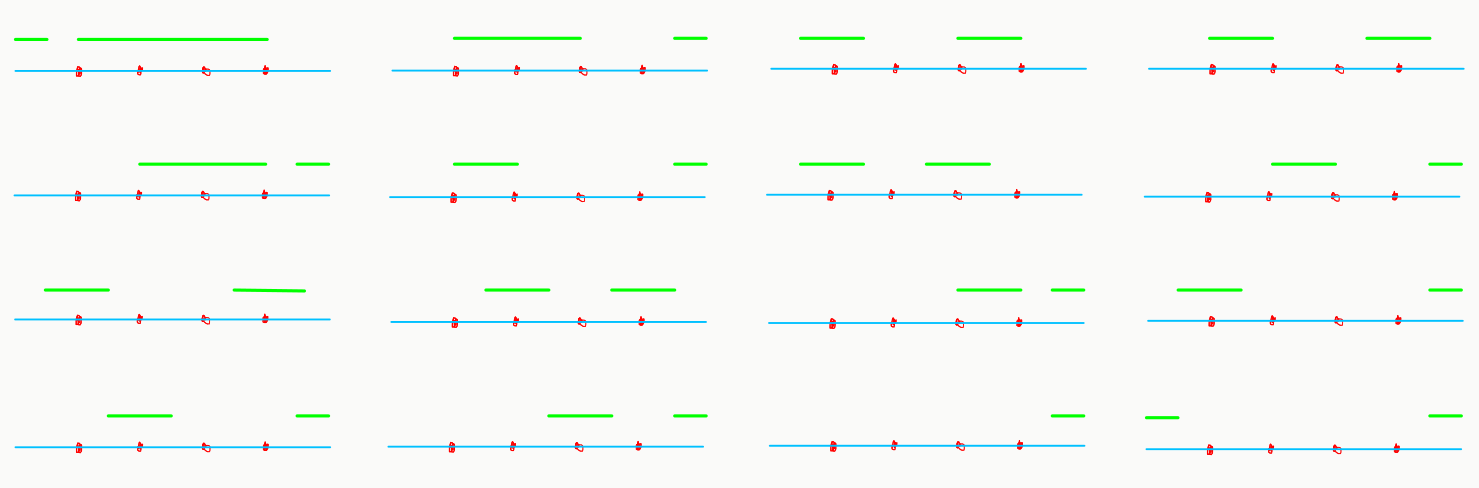
\includegraphics[scale=.4]{intervals.PNG}
			\caption{The VC dimension of pairs of intervals is at least 4.}
	\end{figure}
\end{proof}










\section*{8.3.7}
Let $\mcal{F}$ be the class of indicators of all closed axis-aligned rectangles, i.e. product sets $[a,b]\times [c,d]$ in $\reals^2$. Show that $\vc(\mcal{F}) = 4$.
\begin{proof}
	We can shatter a set of four points in convex position as seen in Figure 2. As for five points, four of them determine a minimal rectangle that encloses all of them: those with the most extreme coordinates. The fifth point must either lie in the interior of this minimal rectangle or it must lie on the boundary. Either way, we can't enclose the four points that determine the minimal rectangle without also enclosing the fifth, so we can't shatter a set of five points.

	\begin{figure}[ht]\label{rectangles}
	\centering
		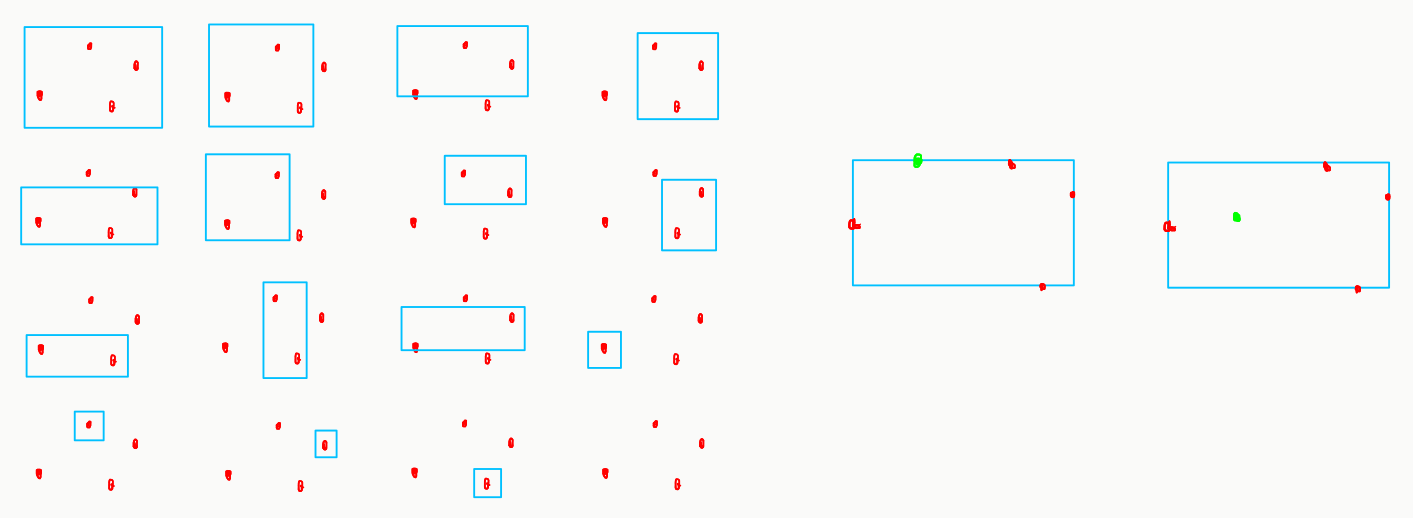
\includegraphics[scale=.4]{rectangles.PNG}	
		\caption{The VC dimension of rectangles is 4.}
	\end{figure}
\end{proof}










\section*{8.3.15}
Recall that Pajor's lemma states that if $\mcal{F}$ is a class of Boolean functions on a finite set $\Omega$, then
\[
|\mcal{F}|\leq |\{\Lambda\subseteq \Omega: \Lambda\text{ is shattered by }\mcal{F}\}|,
\]
where we include the empty set $\Lambda = \emptyset$. Show that this inequality is sharp.
\begin{proof}
	Let $|\Omega| = n$ and let $\mcal{F}$ be the class of boolean functions on $\Omega$ that take the value 1 at most $d$ times, $0\leq d\leq n$. We can imagine $\mcal{F}$ as the set of length $n$ bitstrings with Hamming weight at most $d$. The number of strings with weight $k$ is $\binom{n}{k}$, so
	\[
	|\mcal{F}| = \sum_{k=0}^d\binom{n}{k}.
	\]
	The class $\mcal{F}$ shatters any subset $\Lambda \subseteq \Omega$ with $|\Lambda|\leq d$ since the weight of the bitstrings needed to shatter $\Lambda$ all have weight at most $d$. On the other hand, $\mcal{F}$ doesn't shatter any set of size $d+1$ since it doesn't have any bitstrings with weight $d+1$. The number of shattered sets is then the number of subsets of $\Omega$ with size at most $d$, so
	\[
	|\{\Lambda\subseteq \Omega: \Lambda\text{ is shattered by }\mcal{F}\}| = \sum_{k=0}^d\binom{n}{k}.
	\]
\end{proof}










\section*{8.3.17}
Recall the Sauer-Shelah lemma, which states that if $\mcal{F}$ is a class of Boolean functions on an $n$-point set $\Omega$, then
\[
|\mcal{F}|\leq \sum_{k=0}^d\binom{n}{k}\leq \left(\frac{en}{d}\right)^d,
\]
where $d= \vc(\mcal{F})$. Show that this is sharp for all $n$ and $d$.
\begin{proof}
	We use the same $\Omega$ and $\mcal{F}$ from exercise 8.3.15 -- length $n$ bitstrings with weight at most $d$. In that exercise we showed that
	\[
	|\mcal{F}| = \sum_{k=0}^d\binom{n}{k}.
	\]
	In this example we have that $\vc(\mcal{F}) = d$, so the sharpness of Sauer-Shelah follows.
\end{proof}










\section*{8.3.24}
Let $\mcal{F}$ be a class of functions on a probability space $(\Omega, \Sigma, \mu)$. Let $X, X_1, \ldots, X_n$ be random points in $\Omega$ distributed according to the law $\mu$. Prove that
\[
E\sup_{f\in \mcal{F}}\left|\frac{1}{n}\sum_{i=1}^nf(X_i)-Ef(X)\right|\leq 2E\sup_{f\in \mcal{F}}\left|\frac{1}{n}\sum_{i=1}^n\epsilon_if(X_i)\right|,
\]
where $\epsilon_1, \ldots, \epsilon_n$ are independent symmetric Bernoulli random variables, which are also independent of $X_1, X_2, \ldots$.
\begin{proof}
	Our plan is to modify the proof of Lemma 6.4.2, the symmetrization lemma. Let $X_i'$ be an independent copy of $X_i$, $i=1, \ldots, n$ that is also independent from the $\epsilon_i$'s. Ditto for $X'$. We have
	\begin{align*}
		E\sup_{f\in \mcal{F}}\left|\frac{1}{n}\sum_{i=1}^nf(X_i)-Ef(X)\right| &= E\sup_{f\in \mcal{F}}\left|\frac{1}{n}\sum_{i=1}^nf(X_i)-Ef(X)-E'\frac{1}{n}\sum_{i=1}^nf(X_i')+E'f(X')\right|\\
		&= E\sup_{f\in \mcal{F}}\left|\frac{1}{n}\sum_{i=1}^nf(X_i)-E'\frac{1}{n}\sum_{i=1}^nf(X_i')\right|.
	\end{align*}
	We apply Jensen twice to move the $E'$ out of the absolute value and past the supremum. Since $f(X_i)-f(X_i')$ is symmetric, we bound the above quantity above by
	\begin{align*}
		EE'\sup_{f\in \mcal{F}}\left|\frac{1}{n}\sum_{i=1}^nf(X_i)-\frac{1}{n}\sum_{i=1}^nf(X_i')\right| &= EE'\sup_{f\in \mcal{F}}\left|\frac{1}{n}\sum_{i=1}^n\epsilon_i(f(X_i)-f(X_i'))\right|\\
		&\leq EE'\left[\sup_{f\in \mcal{F}}\left|\frac{1}{n}\sum_{i=1}^n\epsilon_if(X_i)\right| + \sup_{f\in \mcal{F}}\left|\frac{1}{n}\sum_{i=1}^n\epsilon_if(X_i')\right|\right]\\
		&= 2E\sup_{f\in \mcal{F}}\left|\frac{1}{n}\sum_{i=1}^n\epsilon_if(X_i)\right|.
	\end{align*}
\end{proof}










\section*{8.3.25}
In the proof of theorem 8.2.23, we bounded $E\sup_{f\in \mcal{F}}Z_f$ instead of $E\sup_{f\in \mcal{F}}|Z_f|$. Give a bound on the latter quantity.
\begin{solution}
	Let $\mcal{F}_0$ be the class obtained by adding the zero function to $\mcal{F}$. Denote the VC dimension of $\mcal{F}$ by $d$ and that of $\mcal{F}_0$ by $d_0$. Now we write $|Z_f| = |Z_f-Z_0|$, which, when combined with remark 8.1.3 and theorem 8.3.18 gives
	\begin{align*}
		E\sup_{f\in \mcal{F}}|Z_f| \leq E\sup_{f\in \mcal{F}_0}|Z_f-Z_0| &\leq \int_0^1\sqrt{\log N(\mcal{F}_0, L^2_\mu, \epsilon)}d\epsilon\\
		&\leq \int_0^1\sqrt{\log(2/\epsilon)^{Cd_0}}d\epsilon\\
		&= \sqrt{Cd_0}(\log 2+1).
	\end{align*}
	Now we claim that $d_0$ is at most $d+1$. Suppose for the sake of contradiction that $\mcal{F}_0$ shatters a set, $\Lambda$, of size $d+2$. If we remove a point, $x_0$, then $\mcal{F}_0$ must still shatter $\Lambda\setminus \{x_0\}$. Now the subclass $\{f\in \mcal{F}_0: f(x_0)=1\}$ also shatters $\Lambda\setminus \{x_0\}$. But none of these functions are the zero function, so this subclass is also contained in $\mcal{F}$. But then $\mcal{F}$ shatters $\Lambda\setminus \{x_0\}$, which is of size $d+1$. Since this contradicts the assumption that $\vc(\mcal{F})=d$, we conclude that adding the zero function increases the VC dimension of $\mcal{F}$ by at most 1. This gives
	\[
	E\sup_{f\in \mcal{F}}|Z_f|\leq \sqrt{C'(d+1)}.
	\]
\end{solution}










\section*{8.4.8}
Our model of a learning problem postulates that the output $T(X)$ must be completely determined by the input $X$. This is rarely the case in practice. What is more often true is that the output $Y$ is a random variable, which is correlated with the input $X$; the goal of learning is still to predict $Y$ from $X$ as best as possible.\\

Extend the theory of learning up to Theorem 8.4.4 for training data of the form
\[
(X_i, Y_i),\quad i=1, \ldots n
\]
where $(X_i, Y_i)$ are independent copies of a pair $(X,Y)$ consisting of an input random point $X\in \Omega$ and an output random variable $Y$.
\begin{solution}
	Basically, our new goal is to learn the distribution of $Y$ given $X$. We still model our hypothesis as a function $f:\Omega\to \reals$. Since $X$ and $Y$ are both random now, the risk should look something like
	\[
	R(f) = E(f(X)-Y)^2 = \int_{\Omega^2}(f(x)-y)^2\ dP(x,y),
	\]
	where $P(x,y)$ is the joint probability distribution of $X$ and $Y$. Empirical risk looks the same.
	\[
	R_n(f) = \frac{1}{n}\sum_{i=1}^n(f(X_i)-Y_i)^2.
	\]
	The goal should still be to find the hypothesis $f_n^*$ that minimizes the empirical risk.
\end{solution}

\end{document}